\documentclass[12pt]{article}
\textwidth 16.5cm
\textheight 23.5cm
\oddsidemargin 0pt
\topmargin -2cm
\usepackage{epsf}

\usepackage{latexsym,amsmath,amssymb,amsfonts,amsthm,bbm,mathrsfs,breakcites,dsfont,xcolor}
\usepackage{stmaryrd,epsf}
\usepackage{natbib}
\bibliographystyle{plainnat}

\setcitestyle{authoryear, open={(},close={)}}
\usepackage{soul}
\usepackage{url}
\usepackage{dsfont}
\usepackage{enumerate}
\usepackage{graphicx}
\usepackage{graphics}
\usepackage{psfrag}
\usepackage{caption, subcaption}
\usepackage{multirow}
\usepackage[ruled,vlined]{algorithm2e}


\usepackage[colorlinks,linkcolor=black,citecolor=blue,urlcolor=blue,breaklinks = true]{hyperref}

\usepackage[acronym, toc]{glossaries-extra}

\setabbreviationstyle[acronym]{long-short}

\glssetcategoryattribute{acronym}{nohyperfirst}{true}

\renewcommand*{\glsdonohyperlink}[2]{%
 {\glsxtrprotectlinks \glsdohypertarget{#1}{#2}}}

\usepackage{lineno}
% \linenumbers


\newtheorem{theorem}{Theorem}
\newtheorem{lemma}[theorem]{Lemma}
\newtheorem{proposition}[theorem]{Proposition}
\newtheorem{corollary}[theorem]{Corollary}
\newtheorem{assumption}{A\!\!}
\newtheorem{example}{Example}

\DeclareMathOperator*{\argmax}{arg\,max}
\DeclareMathOperator*{\argmin}{arg\,min}
\newcommand{\indep}{\rotatebox[origin=c]{90}{$\models$}}
\newcommand{\red}[1]{\textcolor{red}{#1}}
\newcommand{\blue}[1]{\textcolor{blue}{#1}}
\newcommand{\green}[1]{\textcolor{green}{#1}}
\newcommand{\orange}[1]{\textcolor{orange}{#1}}
\newcommand{\var}{\mathrm{Var}}
\newcommand{\cov}{\mathrm{Cov}}
\newcommand{\bbE}{\mathbb{E}}

\usepackage{xcolor}
\usepackage[draft,inline,nomargin,index]{fixme}
\fxsetup{theme=color,mode=multiuser}
\FXRegisterAuthor{tc}{atc}{\color{red} TC}
\FXRegisterAuthor{jb}{abc}{\color{green} JB}

\newcommand{\vtwo}[1]{\textcolor{red}{#1}}

\makeglossaries 

\newacronym{lasso}{LASSO}{Least Absolute Shrinkage and Selection Operator}
\newacronym{tmb}{TMB}{Tumour Mutation Burden}
\newacronym{tib}{TIB}{Tumour Indel Burden}
\newacronym{icb}{ICB}{Immune Checkpoint Blockade}
\newacronym{ici}{ICI}{Immune Checkpoint Inhibitor}
\newacronym{msi}{MSI}{Micro-Satellite Instability}
\newacronym{ctla4}{CTLA-4}{Cytotoxic T Lymphocyte Associated protein 4}
\newacronym{pdl1}{PD-L1}{Programmed Death Ligand 1}
\newacronym{wes}{WES}{Whole Exome Sequencing}
\newacronym{ctdna}{ctDNA}{Circulating Tumour DNA}
\newacronym{bmr}{BMR}{Background Mutation Rate}
\newacronym{nsclc}{NSCLC}{Non-Small Cell Lung Cancer}
\newacronym{auprc}{AUPRC}{area under the precision-recall curve}
\newacronym{ectmb}{ecTMB}{Estimation and Classification of Tumour Mutation Burden}

\title{Additional figures for revisions}
\begin{document}
\section{Multi-cancer analysis}
\subsection{Three-cancer comparisons versions of figures 6 and 8}
See Figure~\ref{fig:joint_versions_figs68}. Broadly speaking, decreasing performance for decreasing levels of average \gls{tmb}. Since 0.6Mb panel size was selected in advance (from NSCLC study), only train and test split (no val). For SKCM: $n_{\text{train}} = 250$, $n_{\text{test}} = 96$. For COADREAD: $n_{\text{train}} = 500$, $n_{\text{test}} = 119$. For BLCA: $n_{\text{train}} = 300$, $n_{\text{test}} = 109$. Note that the quality of predictions doesn't seem to be particularly dependent on training sample size, and far more so on average \gls{tmb} value (SKCM: 570, COADREAD: 330, BLCA: 250). \jbnote{Get rid of right hand side. Get rid of dashed lines on left hand side. Include blue line on left hand side that shows performance on external validation set.}
\begin{figure}[h]
    \centering
    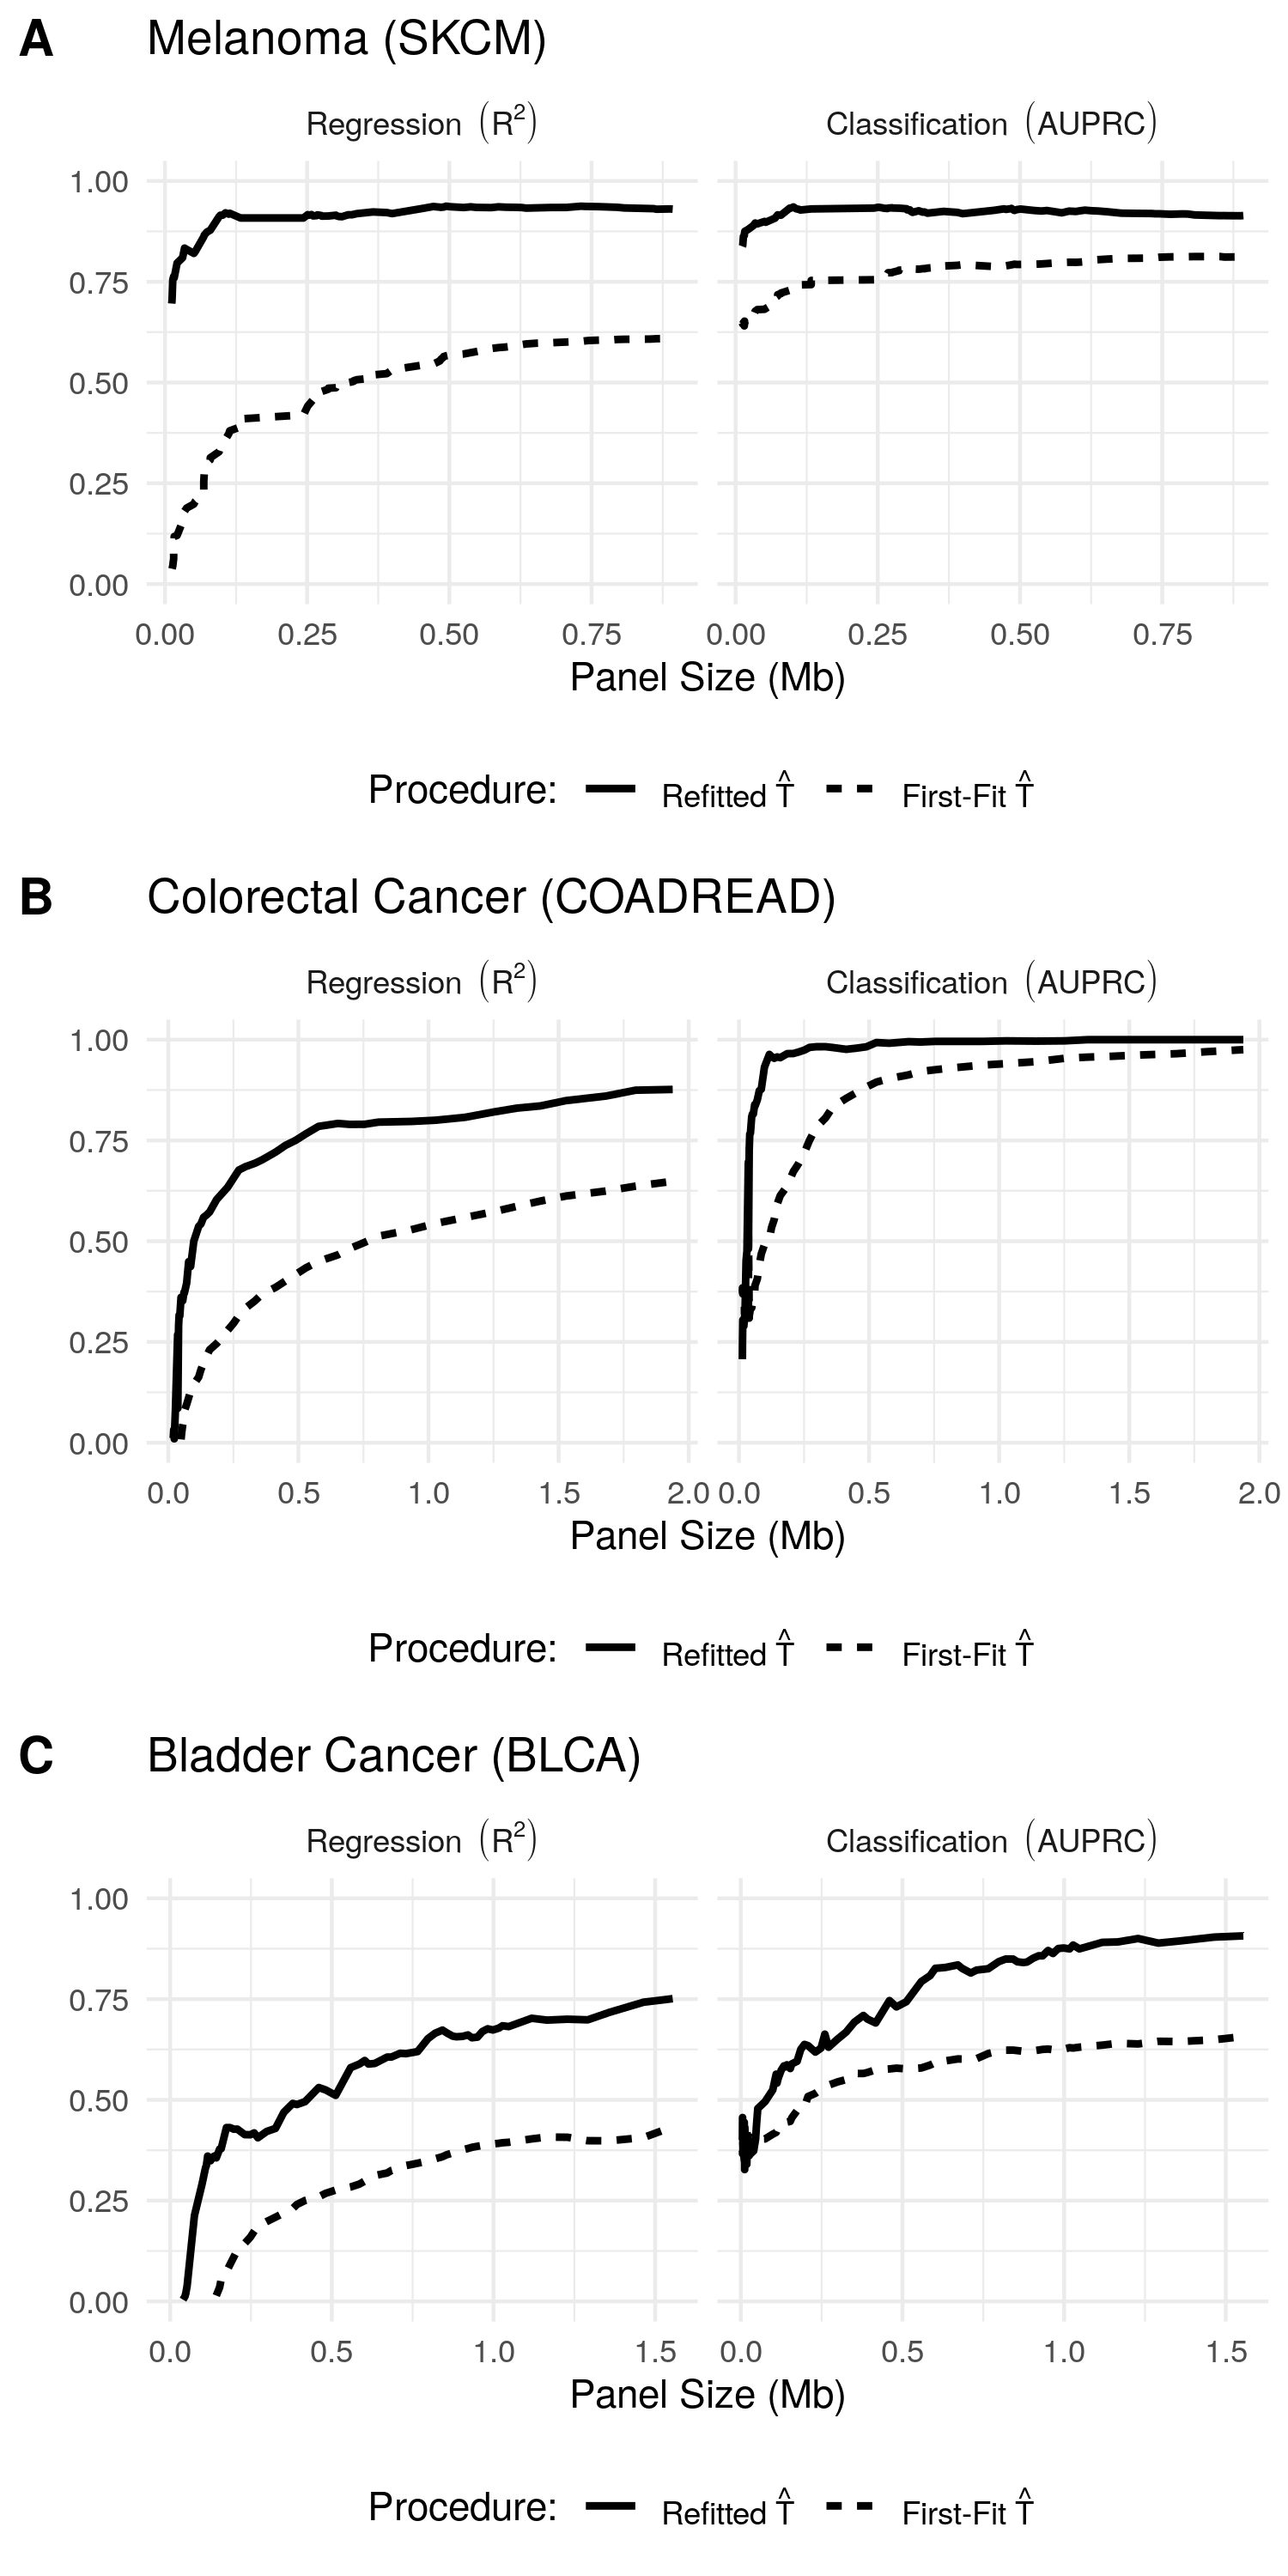
\includegraphics[width=3in]{results/figures/joint_version_fig6.png} \hspace{5pt}
    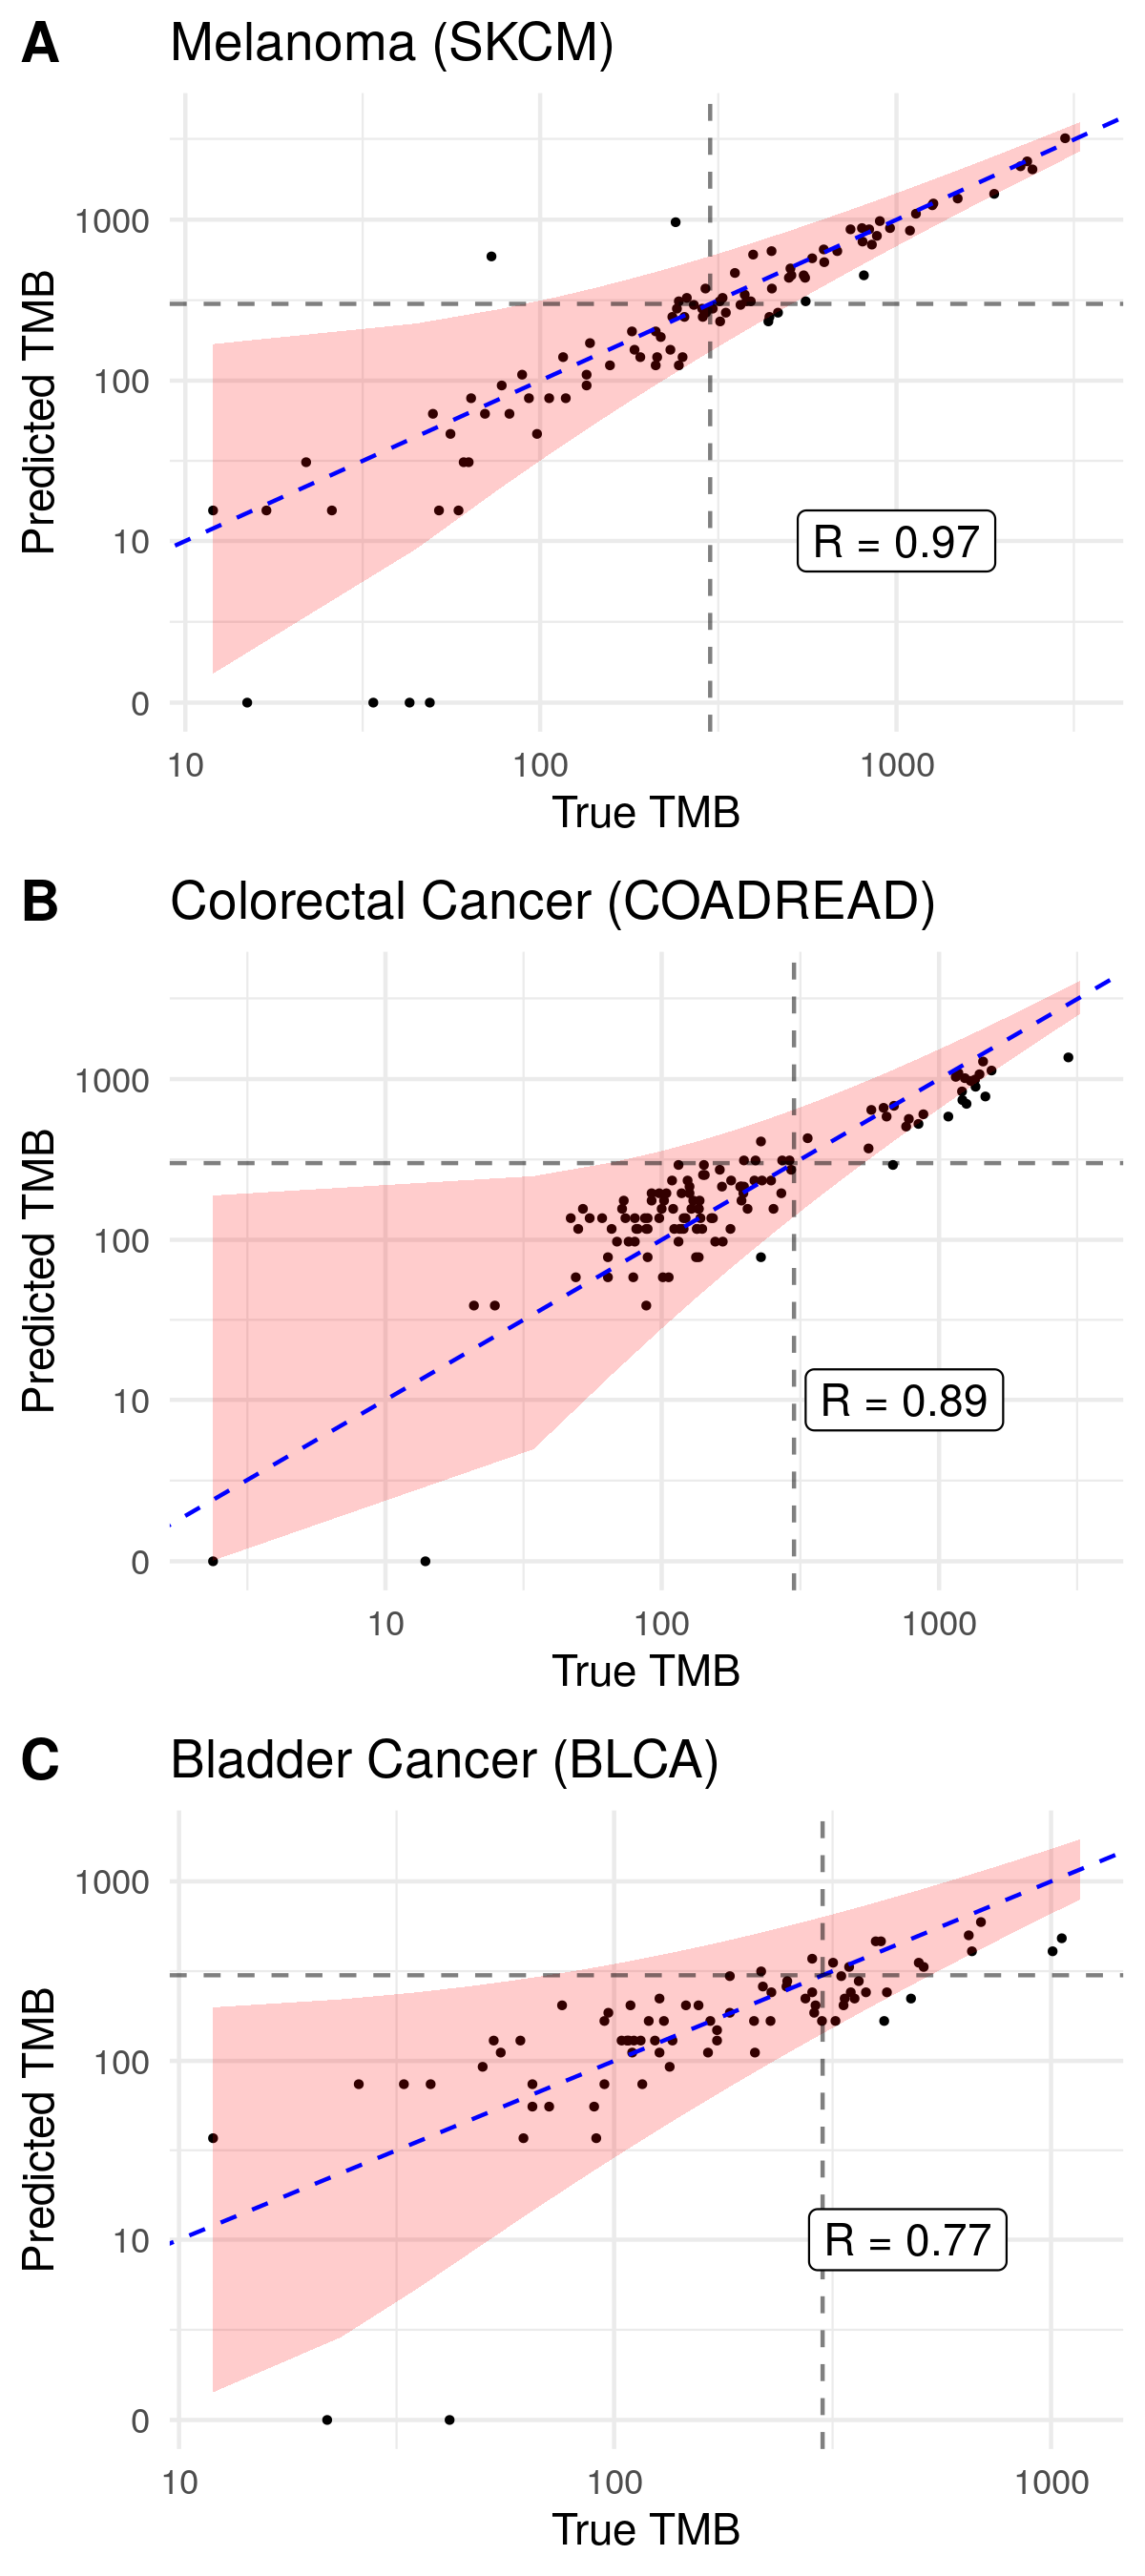
\includegraphics[width=2.7in]{results/figures/joint_version_fig8.png}
    \caption{\textbf{Left}: Test set panel performances for a range of panel sizes, each of three cancer types. \textbf{Right}: True versus predicted TMB for 0.6Mb selected panel on test set, each of three cancer types.
    \label{fig:joint_versions_figs68}}
\end{figure}
\newpage
\subsection{Survival analysis in external study (MSK-IMPACT panel)}
See Figure~\ref{fig:msk_forests}. Very little difference between hazard ratios for study derived

\begin{figure}[h]
    \centering
    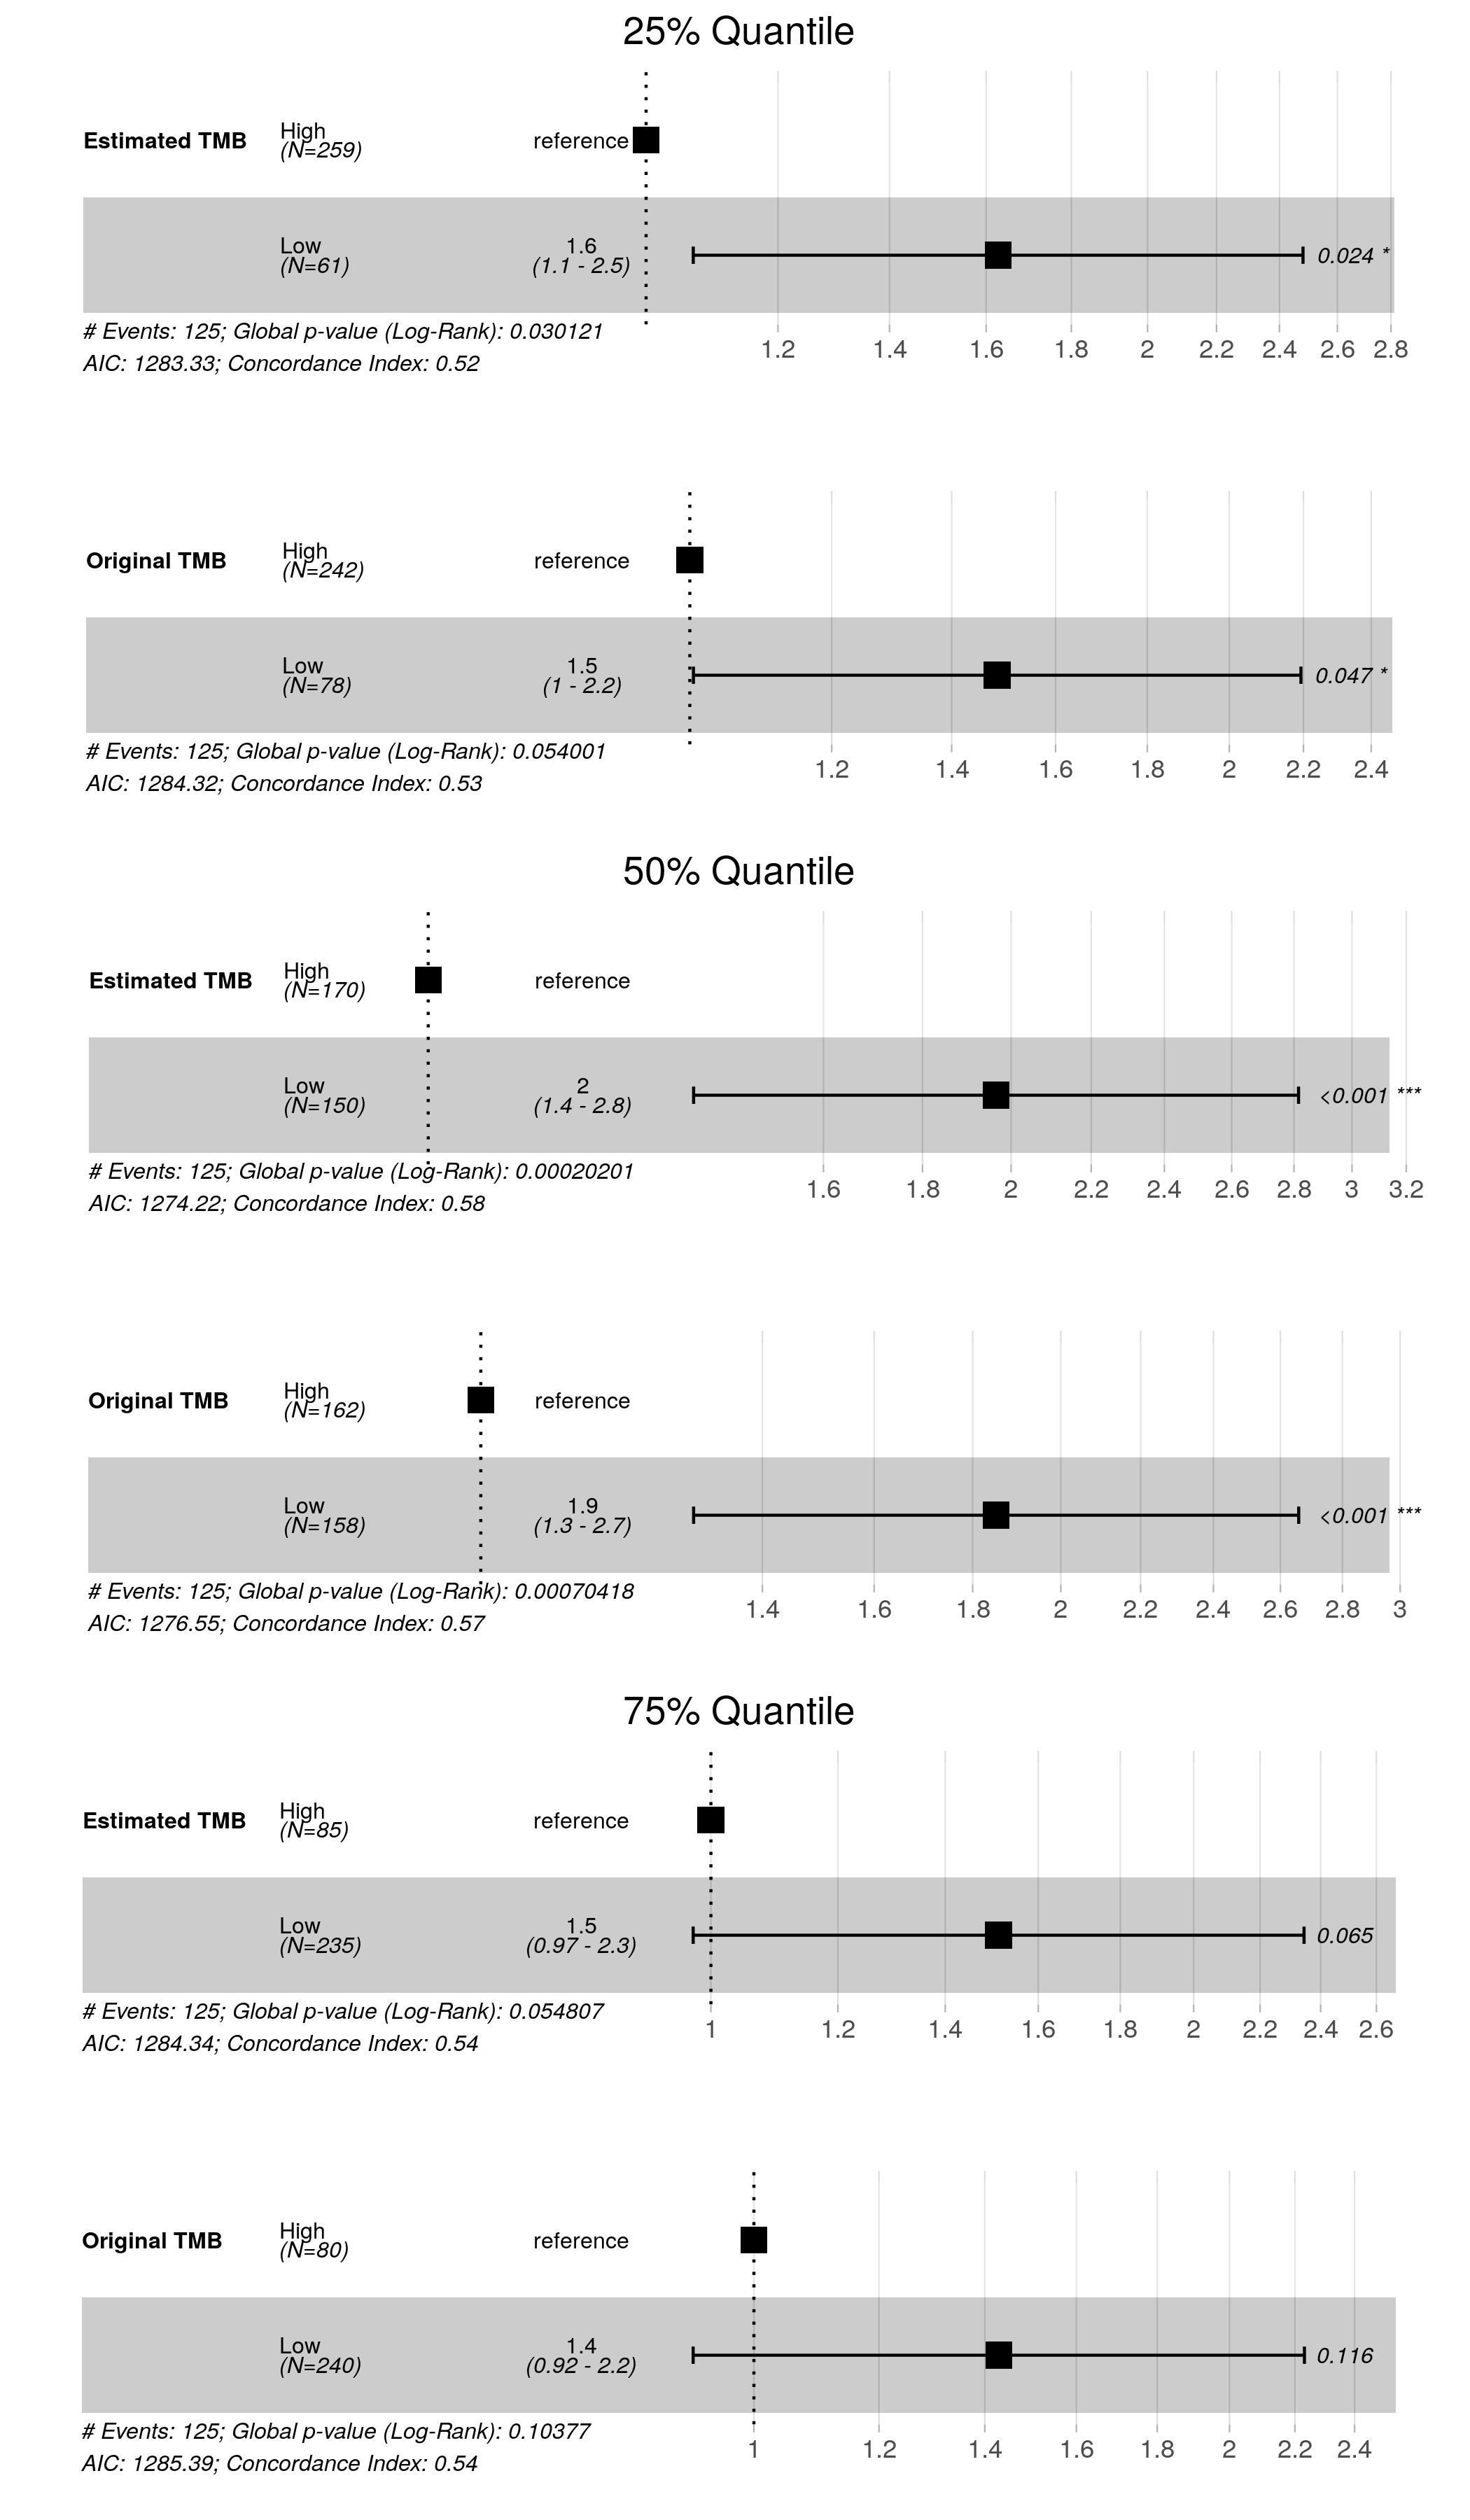
\includegraphics[width=2.5in]{results/figures/skcm_forests.png}
    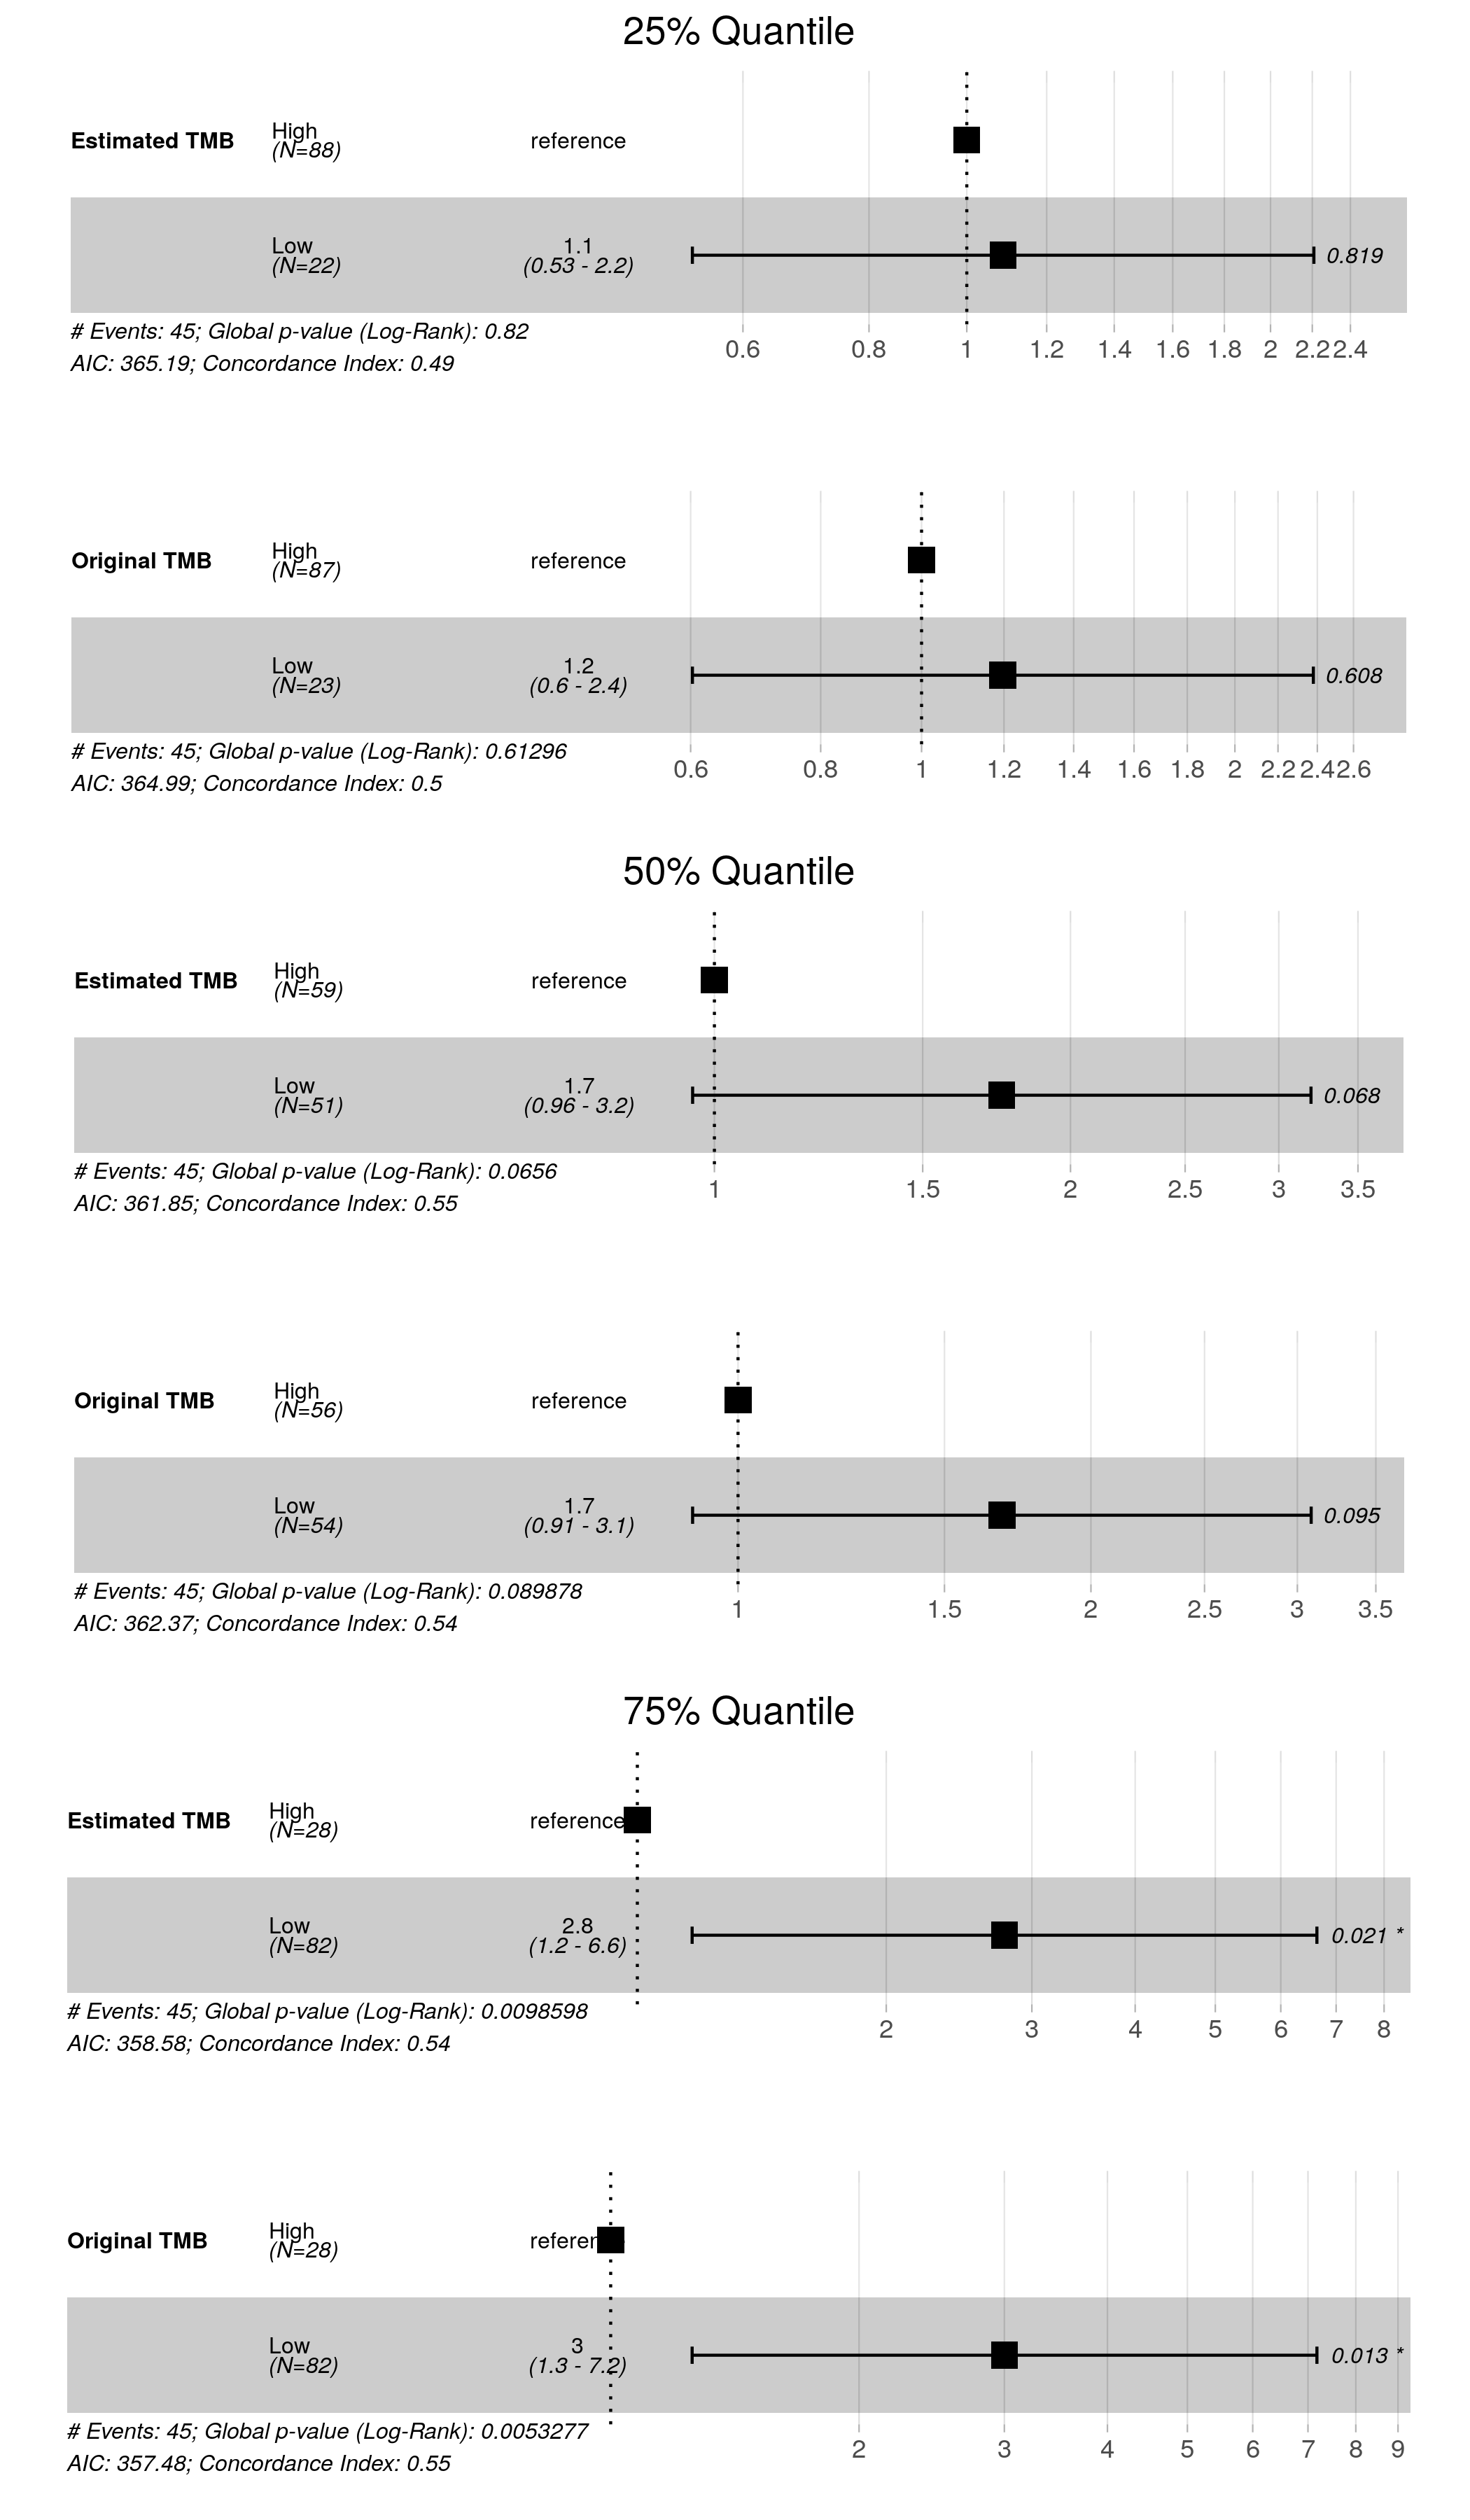
\includegraphics[width=2.5in]{results/figures/coadread_forests.png}
    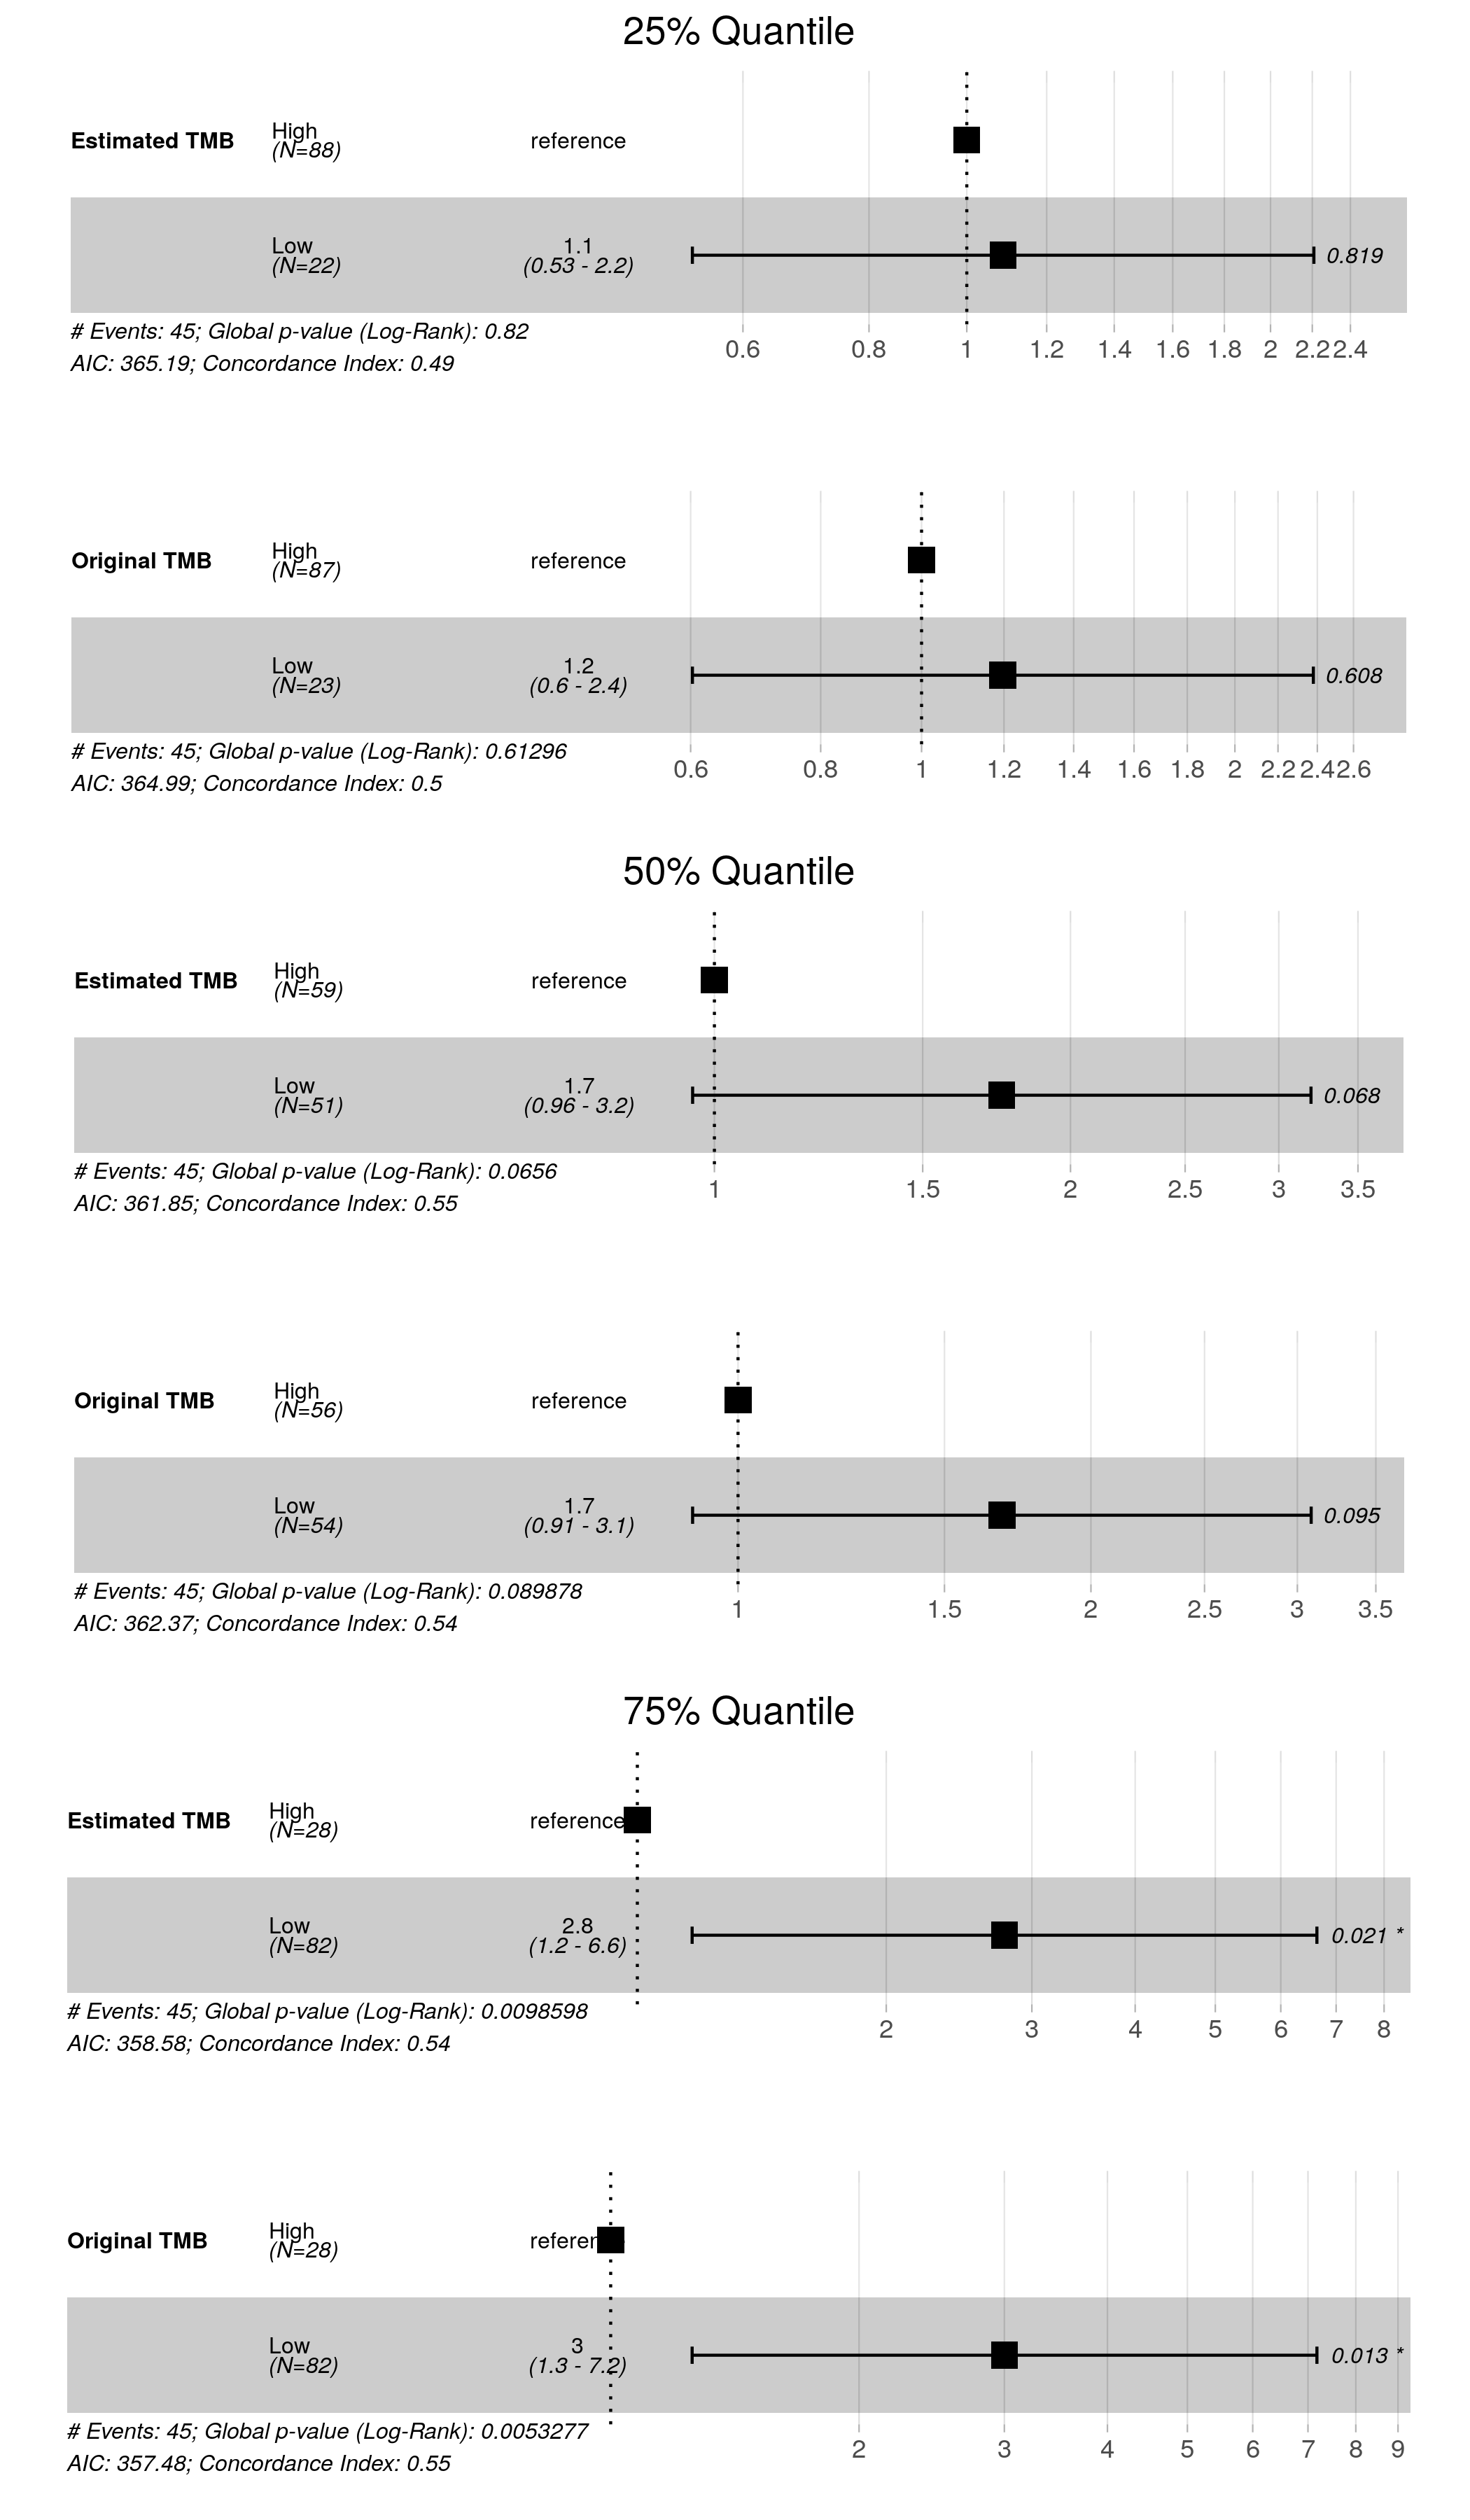
\includegraphics[width=2.5in]{results/figures/blca_forests.png}
    \caption{Hazard ratios of estimated verus study derived TMB status, for TMB-High defined at 25\%, 50\% and 75\% quantiles. \textbf{Top left}: SKCM \textbf{Top Right}: COADREAD \textbf{Bottom}: BLCA.}
    \label{fig:msk_forests}
\end{figure}

\end{document}